\documentclass{article}

\usepackage{amsmath}
\usepackage{amssymb}
\usepackage{algorithm}
\usepackage[noend]{algpseudocode}		% for algorithms in pseudo code. Usage: \begin{algorithmic}
\MakeRobust{\Call}
\usepackage{tikz}	% for diagrams
\usetikzlibrary{positioning}
\usetikzlibrary{quotes}
% Math mode in tables
\usepackage{array}   % for \newcolumntype macro
\newcolumntype{C}{>{$}c<{$}} % math-mode version of "c" column type

\setlength{\parskip}{\smallskipamount}

\title{Analysis of Algorithms \\
\medskip
\large Homework 5 -- Networks}
\author{Abraham Murciano}

\begin{document}

\maketitle

\section*{Question 1}

\subsection*{Part A}

We are given the network in figure \ref{q1}. We are to find the maximal flow using the Edmonds-Karp algorithm.

\begin{figure}[htbp]
	\centering
	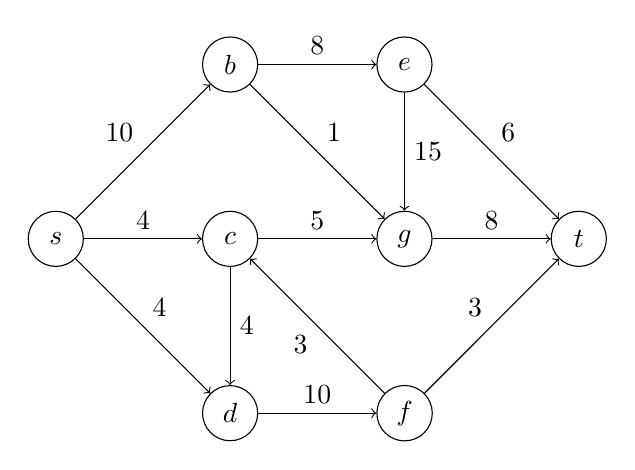
\begin{tikzpicture}
		[vertex/.style={circle, draw=black, node distance=1.5cm, minimum size=0.7cm}]
		\node[vertex] (s) {\(s\)};
		\node[vertex, right=of s] (c) {\(c\)};
		\node[vertex, above=of c] (b) {\(b\)};
		\node[vertex, below=of c] (d) {\(d\)};
		\node[vertex, right=of b] (e) {\(e\)};
		\node[vertex, right=of d] (f) {\(f\)};
		\node[vertex, right=of c] (g) {\(g\)};
		\node[vertex, right=of g] (t) {\(t\)};

		\draw[->] (s) to["10"] (b);
		\draw[->] (s) to["4"] (c);
		\draw[->] (s) to["4"] (d);
		\draw[->] (c) to["4"] (d);
		\draw[->] (b) to["8"] (e);
		\draw[->] (b) to["1"] (g);
		\draw[->] (e) to["15"] (g);
		\draw[->] (c) to["5"] (g);
		\draw[->] (d) to["10"] (f);
		\draw[->] (f) to["3"] (c);
		\draw[->] (f) to["3"] (t);
		\draw[->] (g) to["8"] (t);
		\draw[->] (e) to["6"] (t);
	\end{tikzpicture}
	\caption{A network}
	\label{q1}
\end{figure}

The first augmenting path which the algorithm finds can be \((s, b, e, t)\) (it may vary depending on the order that neighbours are selected in the BFS), through which a flow of 6 can be sent. The states of the graph at each point are shown in figure \ref{q1-steps}. (Saturated edges are omitted, and only remaining capacity is shown on each edge.)

The next augmenting path could be \((s, b, g, t)\) with a flow of 1. After this one, another possible augmenting path is \((a, c, g, t)\), which has a flow of 4. Next is \((s, d, f, t)\) with a flow of 3. The next augmenting path is \(s, b, e, g, t\). A flow of 2 can be sent through this one. The final augmenting path has a flow of 1, and is \((s, d, f, c, g, t)\).

Once there are no more augmenting paths to be found, we can sum up the flows through all the augmenting paths to find the maximal flow, which for this network is \(6 + 1 + 4 + 3 + 2 + 1 = 17\).

\begin{figure}[htbp]
	\centering
	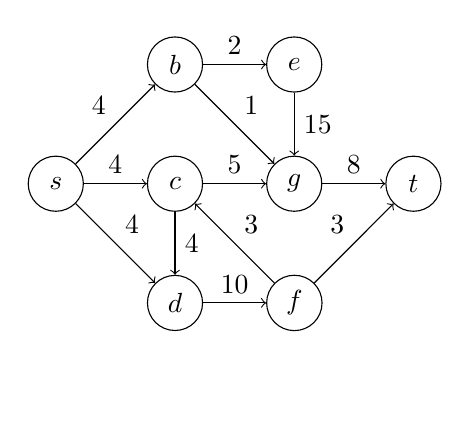
\begin{tikzpicture}
		[vertex/.style={circle, draw=black, node distance=0.8cm, minimum size=0.7cm, minimum size=0.7cm}]
		\node[vertex] (s) {\(s\)};
		\node[vertex, right=of s] (c) {\(c\)};
		\node[vertex, above=of c] (b) {\(b\)};
		\node[vertex, below=of c] (d) {\(d\)};
		\node[vertex, right=of b] (e) {\(e\)};
		\node[vertex, right=of d] (f) {\(f\)};
		\node[vertex, right=of c] (g) {\(g\)};
		\node[vertex, right=of g] (t) {\(t\)};
		\node[below=0.6cm of d]{};

		\draw[->] (s) to["4"] (b);
		\draw[->] (s) to["4"] (c);
		\draw[->] (s) to["4"] (d);
		\draw[->] (c) to["4"] (d);
		\draw[->] (b) to["2"] (e);
		\draw[->] (b) to["1"] (g);
		\draw[->] (e) to["15"] (g);
		\draw[->] (c) to["5"] (g);
		\draw[->] (d) to["10"] (f);
		\draw[->] (f) to["3" above right] (c);
		\draw[->] (f) to["3"] (t);
		\draw[->] (g) to["8"] (t);
	\end{tikzpicture}
	\hfill
	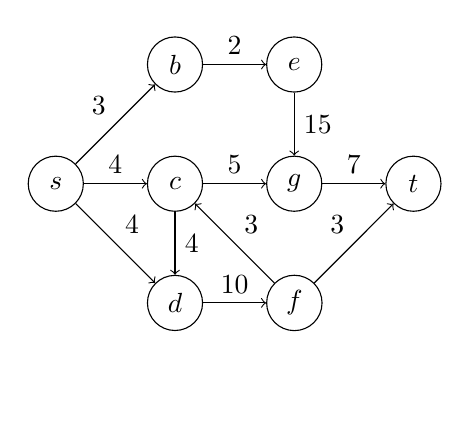
\begin{tikzpicture}
		[vertex/.style={circle, draw=black, node distance=0.8cm, minimum size=0.7cm}]
		\node[vertex] (s) {\(s\)};
		\node[vertex, right=of s] (c) {\(c\)};
		\node[vertex, above=of c] (b) {\(b\)};
		\node[vertex, below=of c] (d) {\(d\)};
		\node[vertex, right=of b] (e) {\(e\)};
		\node[vertex, right=of d] (f) {\(f\)};
		\node[vertex, right=of c] (g) {\(g\)};
		\node[vertex, right=of g] (t) {\(t\)};
		\node[below=0.6cm of d]{};

		\draw[->] (s) to["3"] (b);
		\draw[->] (s) to["4"] (c);
		\draw[->] (s) to["4"] (d);
		\draw[->] (c) to["4"] (d);
		\draw[->] (b) to["2"] (e);
		\draw[->] (e) to["15"] (g);
		\draw[->] (c) to["5"] (g);
		\draw[->] (d) to["10"] (f);
		\draw[->] (f) to["3" above right] (c);
		\draw[->] (f) to["3"] (t);
		\draw[->] (g) to["7"] (t);
	\end{tikzpicture}

	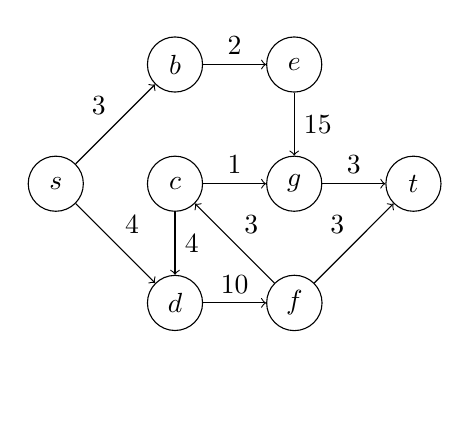
\begin{tikzpicture}
		[vertex/.style={circle, draw=black, node distance=0.8cm, minimum size=0.7cm}]
		\node[vertex] (s) {\(s\)};
		\node[vertex, right=of s] (c) {\(c\)};
		\node[vertex, above=of c] (b) {\(b\)};
		\node[vertex, below=of c] (d) {\(d\)};
		\node[vertex, right=of b] (e) {\(e\)};
		\node[vertex, right=of d] (f) {\(f\)};
		\node[vertex, right=of c] (g) {\(g\)};
		\node[vertex, right=of g] (t) {\(t\)};
		\node[below=0.6cm of d]{};

		\draw[->] (s) to["3"] (b);
		\draw[->] (s) to["4"] (d);
		\draw[->] (c) to["4"] (d);
		\draw[->] (b) to["2"] (e);
		\draw[->] (e) to["15"] (g);
		\draw[->] (c) to["1"] (g);
		\draw[->] (d) to["10"] (f);
		\draw[->] (f) to["3" above right] (c);
		\draw[->] (f) to["3"] (t);
		\draw[->] (g) to["3"] (t);
	\end{tikzpicture}
	\hfill
	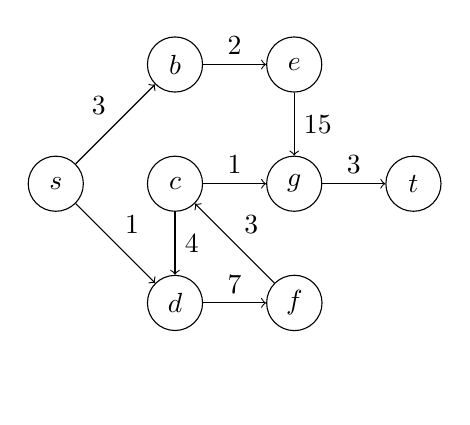
\begin{tikzpicture}
		[vertex/.style={circle, draw=black, node distance=0.8cm, minimum size=0.7cm}]
		\node[vertex] (s) {\(s\)};
		\node[vertex, right=of s] (c) {\(c\)};
		\node[vertex, above=of c] (b) {\(b\)};
		\node[vertex, below=of c] (d) {\(d\)};
		\node[vertex, right=of b] (e) {\(e\)};
		\node[vertex, right=of d] (f) {\(f\)};
		\node[vertex, right=of c] (g) {\(g\)};
		\node[vertex, right=of g] (t) {\(t\)};
		\node[below=0.6cm of d]{};

		\draw[->] (s) to["3"] (b);
		\draw[->] (s) to["1"] (d);
		\draw[->] (c) to["4"] (d);
		\draw[->] (b) to["2"] (e);
		\draw[->] (e) to["15"] (g);
		\draw[->] (c) to["1"] (g);
		\draw[->] (d) to["7"] (f);
		\draw[->] (f) to["3" above right] (c);
		\draw[->] (g) to["3"] (t);
	\end{tikzpicture}

	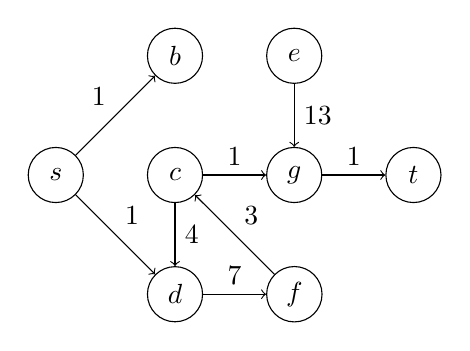
\begin{tikzpicture}
		[vertex/.style={circle, draw=black, node distance=0.8cm, minimum size=0.7cm}]
		\node[vertex] (s) {\(s\)};
		\node[vertex, right=of s] (c) {\(c\)};
		\node[vertex, above=of c] (b) {\(b\)};
		\node[vertex, below=of c] (d) {\(d\)};
		\node[vertex, right=of b] (e) {\(e\)};
		\node[vertex, right=of d] (f) {\(f\)};
		\node[vertex, right=of c] (g) {\(g\)};
		\node[vertex, right=of g] (t) {\(t\)};

		\draw[->] (s) to["1"] (b);
		\draw[->] (s) to["1"] (d);
		\draw[->] (c) to["4"] (d);
		\draw[->] (e) to["13"] (g);
		\draw[->] (c) to["1"] (g);
		\draw[->] (d) to["7"] (f);
		\draw[->] (f) to["3" above right] (c);
		\draw[->] (g) to["1"] (t);
	\end{tikzpicture}
	\hfill
	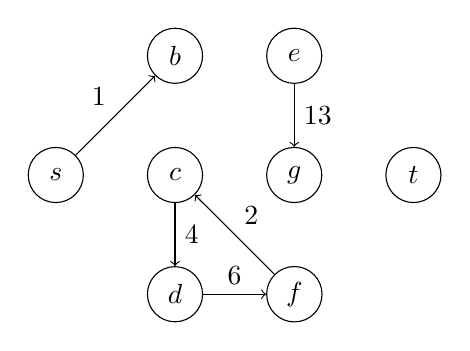
\begin{tikzpicture}
		[vertex/.style={circle, draw=black, node distance=0.8cm, minimum size=0.7cm}]
		\node[vertex] (s) {\(s\)};
		\node[vertex, right=of s] (c) {\(c\)};
		\node[vertex, above=of c] (b) {\(b\)};
		\node[vertex, below=of c] (d) {\(d\)};
		\node[vertex, right=of b] (e) {\(e\)};
		\node[vertex, right=of d] (f) {\(f\)};
		\node[vertex, right=of c] (g) {\(g\)};
		\node[vertex, right=of g] (t) {\(t\)};

		\draw[->] (s) to["1"] (b);
		\draw[->] (c) to["4"] (d);
		\draw[->] (e) to["13"] (g);
		\draw[->] (d) to["6"] (f);
		\draw[->] (f) to["2" above right] (c);
	\end{tikzpicture}
	\caption{The stages of the graph after sending sending flow through each shortest path}
	\label{q1-steps}
\end{figure}

\subsection*{Part B}

The minimal cut in the network must be a cut such that the sum of the capacities of the forward facing edges is minimal. We know however, that the capacity of the minimal cut must always be the same as the maximal flow. Therefore a minimal cut of the network in figure \ref{q1} must have a capacity of 17. One such cut is the following one.
\begin{equation*}
	(\{s, b\}, \{c, d, e, f, g, t\})
\end{equation*}

\section*{Question 2}

\subsection*{Part A}

Supposing we have a network \(N\), we are told that \(N'\) is a modified version of \(N\) such that all the capacities of \(N\) are multiplied by some constant \(c > 1\). If \(f_{\max}\) and \(f'_{\max}\) are the maximal flows of \(N\) and \(N'\) respectively, then \(f'_{\max} = cf_{\max}\)

To demonstrate this, suppose \(P\) is the set of all augmenting paths found by a run of the Edmonds-Karp algorithm on either \(N\) or \(N'\) (\(P\) would be the same regardless of which network is used).

Now for any \(p \in P\), we will denote by \(f_p\) and \(f'_p\) the amount of flow that can be sent through \(p\) on the networks \(N\) and \(N'\) respectively. This is equal to the smallest capacity of an edge along the path \(p\). But since all the capacities in \(N'\) are \(c\) multiplied by the corresponding capacity in \(N\), it follows that \(f'_p = cf_p\).

Finally, we know the following.

\begin{gather*}
	f_{\max} = \sum_{p \in P} f_p \\
	f'_{\max} = \sum_{p \in P} f'_p = \sum_{p \in P} cf_p = c \sum_{p \in P} f_p = cf_{\max} \\
\end{gather*}

\subsection*{Part B}

If we tweak the problem in part A such that \(0 < c < 1\), the answer would be the same, with the same explanation, because the explanation given for part A at no point applies the assumption that \(c > 1\). It holds for all \(c > 0\).

\section*{Question 3}

We are tasked with finding a maximal set of disjoint paths for the graph in figure \ref{q3} from vertices 1 to 6. The maximal set for this graph is the set \(\{p_1, p_2, p_3\}\), such that:

\begin{gather*}
	p_1 = ((1,2), (2,6)) \\
	p_2 = ((1,5), (5,6)) \\
	p_3 = ((1,8), (8,7), (7,6))
\end{gather*}

\begin{figure}[htbp]
	\centering
	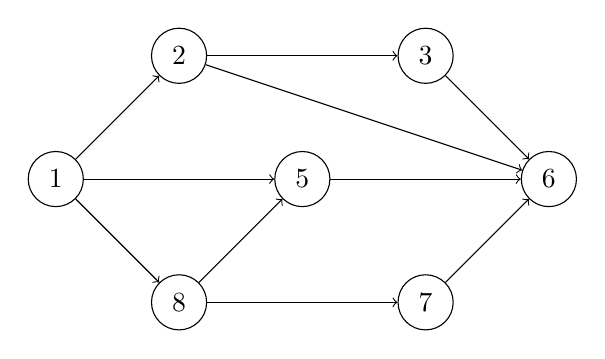
\begin{tikzpicture}
		[vertex/.style={circle, draw=black, node distance=1.5cm, minimum size=0.7cm}]
		\node[vertex] (a) {1};
		\node[vertex, above right=of a] (b) {2};
		\node[vertex, below right=of a] (h) {8};
		\node[vertex, below right=of b] (e) {5};
		\node[vertex, above right=of e] (c) {3};
		\node[vertex, below right=of e] (g) {7};
		\node[vertex, below right=of c] (f) {6};

		\draw[->] (a) to (b);
		\draw[->] (a) to (e);
		\draw[->] (a) to (h);
		\draw[->] (h) to (e);
		\draw[->] (b) to (c);
		\draw[->] (h) to (g);
		\draw[->] (b) to (f);
		\draw[->] (c) to (f);
		\draw[->] (e) to (f);
		\draw[->] (g) to (f);
	\end{tikzpicture}
	\caption{A sample graph for question 3}
	\label{q3}
\end{figure}

\subsection*{Part B}

We are to suggest an algorithm based on maximal flow that will find a maximal set of disjoint paths from \(s\) to \(t\) given a directed graph.

If we construct a network out of the given graph, such that the capacities of each edge are all some constant \(c\), then we attempt to find the maximal flow using the Ford–Fulkerson method, we can return a set of all augmenting paths as the maximal set of disjoint paths.

This set must be disjoint, because once an edge has been used with a flow of \(c\), it is saturated and will not be used as part of another augmenting path. This set must also me maximal because we can send \(c\) units of flow through each augmenting path, so the maximal flow must be sent through the maximal number of augmenting paths.

\section*{Question 4}

Suppose that for a network, in addition to capacities being assigned to edges, capacity is also assigned to each vertex, so that maximal flow that can pass through vertex \(v\) is \(c_v\).

We are to suggest an algorithm to find maximal flow through this network, specifying its run-time complexity.

We can calculate the maximal flow of such a network by replacing each vertex \(v\) by two vertices \(v_1\) and \(v_2\). Then each edge of the form \((x, v)\) or \((v, y)\) is replaced with \((x, v_1)\) and \((v_2, y)\) respectively. We then add a single edge \((v_1, v_2)\) with the capacity \(c_v\). Thus we translate all the vertex capacities into edge capacities, transforming our problem into one we can already solve.

The preprocessing stage can be done in \(O(|V|+|E|)\), and then if we use the Edmonds-Karp algorithm for the next stage, the total complexity would be that of the Edmonds-Karp algorithm; i.e. \(O(|V||E|^2)\).

\end{document}